% !TEX program = xelatex
% ¡Recuerda compilar con XeLaTeX o LuaLaTeX!
\documentclass{article}

% --- Cargar nuestro fichero de estilo ---
% Se asume que paper_style.sty está disponible o se usan paquetes estándar.
\usepackage{paper_style}

% --- PAQUETES PARA EL CONTENIDO DEL DOCUMENTO ---
\usepackage{graphicx}
\usepackage{subcaption}
\usepackage{amsmath}
\usepackage{booktabs}
\usepackage{geometry}
\usepackage{hyperref}
\usepackage{enumitem}
\usepackage{float}



% --- Información del Paper ---
\title{Informe: \\ Introducción a la Consola de Administración de AWS}
\author{
	Jordi Blasco Lozano \\
	\small Infraestructuras y Servicios Cloud \\
	\small Universidad de Alicante
}
\date{\today}

% --- Comienzo del Documento ---
\begin{document}
	
	\maketitle

	\begin{abstract}
	\noindent En esta práctica veremos como lanzar un servidor Apache con un html dentro de una instancia, como replicar instancias gracias a las AMIs, como configurar un balanceador de carga para redirigir el trafico entre varias instancias y todo esto siguiendo unas pautas y un orden para poder llegar a tener el siguiente esquema como sistema en funcionamiento.
	\end{abstract}
	\begin{figure}[H]
	\centering
	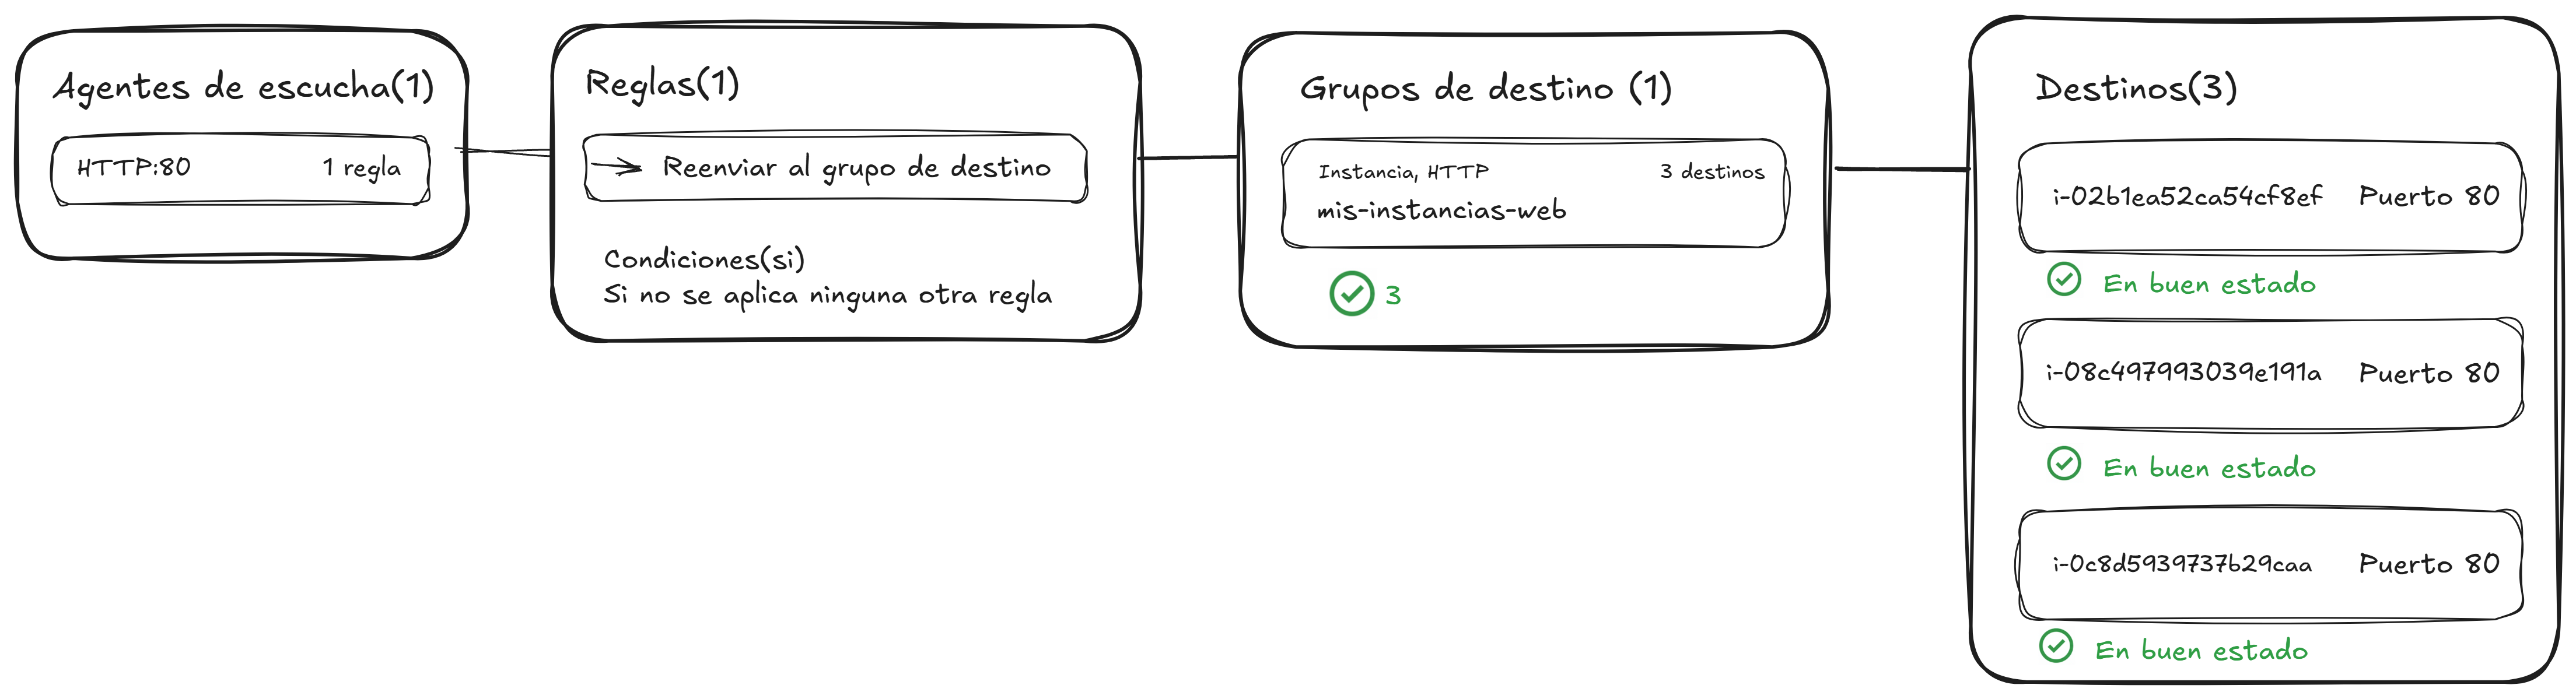
\includegraphics[width=0.95\textwidth]{esquema.png}
	\end{figure}


	\tableofcontents

	\newpage

	\section{Creación de la instancia base}

		Para poder tener la pagina web desplegada debemos de iniciar la primera instancia. Esta primera instancia vendrá de una imagen limpia de Amazon Linux. Nos conectaremos mediante ssh a la instancia para instalar httpd y poder cargar el html copiando con nano.

	\subsection{Configuración de red}

		Para poder acceder a nuestro servidor mediante una url debemos de configurar la instancia de forma que permita accesos http y https. Esto lo haremos mediante la creación de un grupo de seguridad personalizado en el cual permitamos accesos http y https desde cualquier lugar.

	\begin{figure}[H]
	\centering
	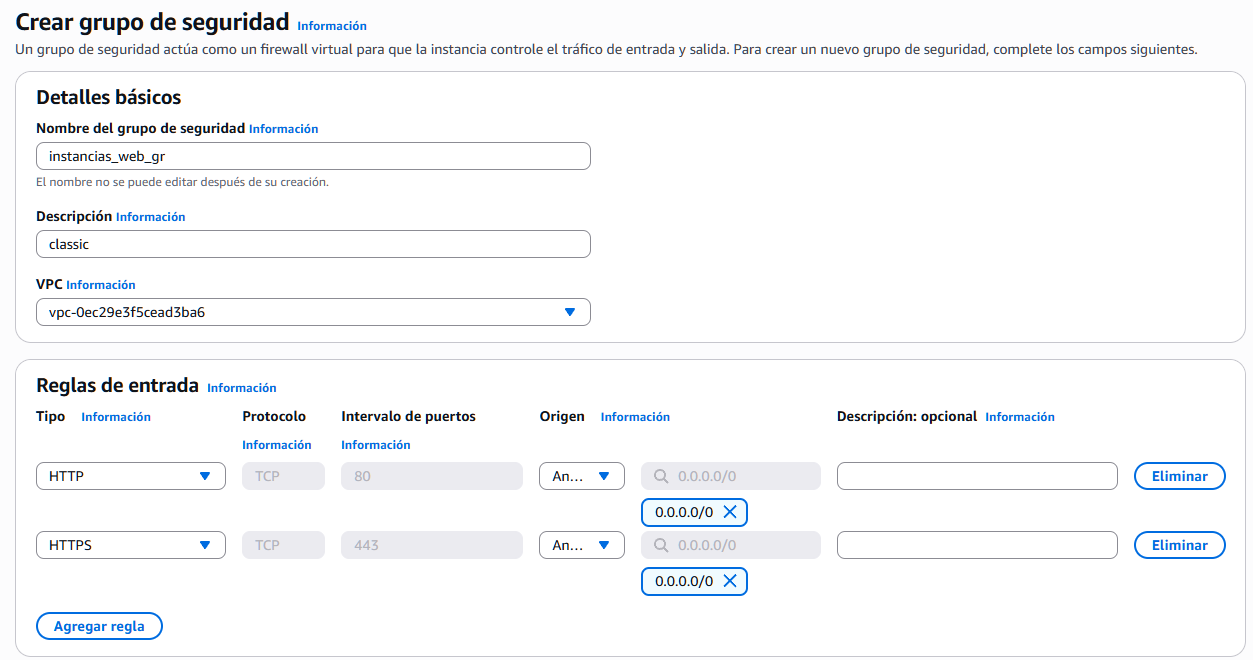
\includegraphics[width=0.95\textwidth]{crear_grupo_seguridad.png}
	\caption{panel de crear grupo de seguridad}
	\end{figure}

	\begin{figure}[H]
	\centering
	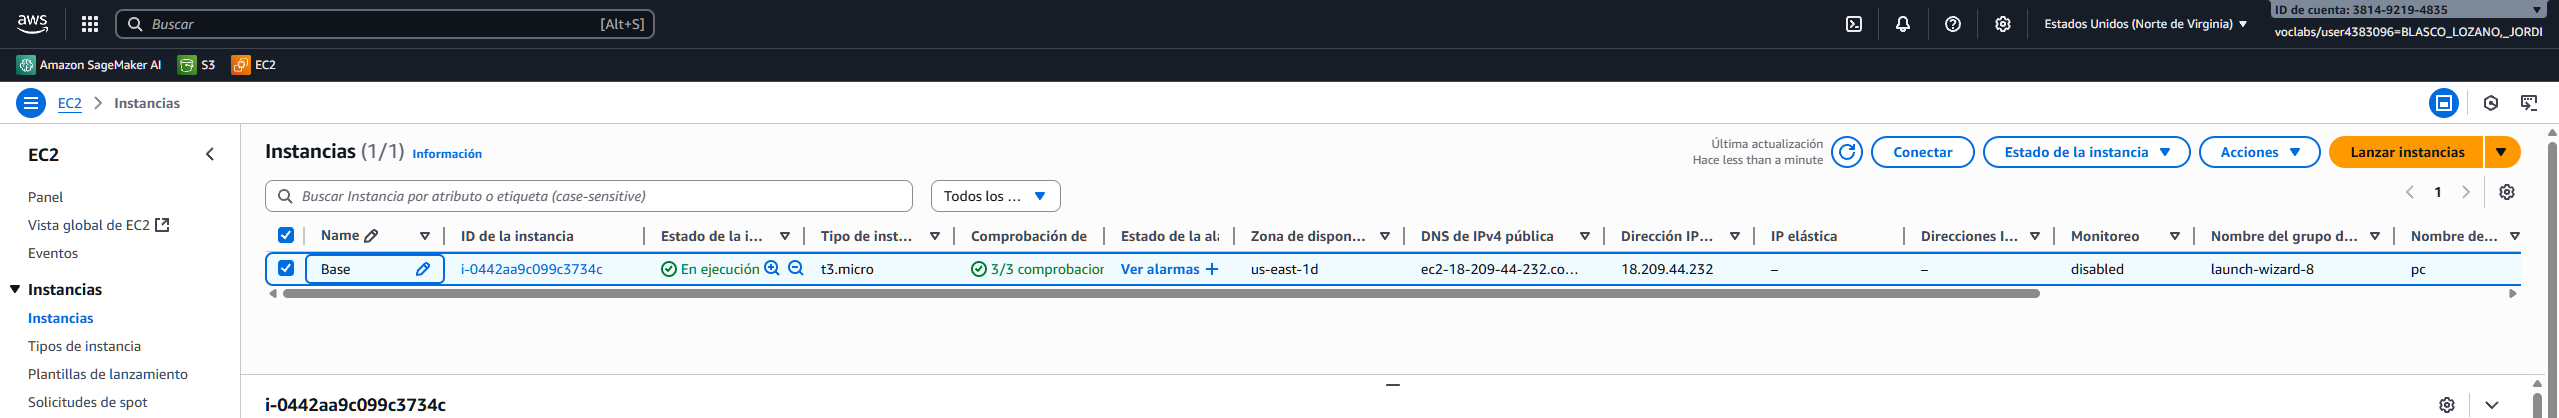
\includegraphics[width=0.95\textwidth]{pestanya_instancias.png}
	\caption{Panel de instancias}
	\end{figure}
\newpage

	\subsection{Instalación de dependencias}

		Una vez tengamos la instancia creada deberemos de conectarnos a ella por ssh. Cuando estemos dentro de la instancia instalaremos httpd mediante el comando sudo yum install httpd. httpd es un servidor web Apache que utilizaremos para desplegar nuestro index.html.


\begin{lstlisting}[style=consola, language=bash, caption={Terminal, dependencias}]
   ,     #_
   ~\_  ####_        Amazon Linux 2023
  ~~  \_#####\
  ~~     \###|
  ~~       \#/ ___   https://aws.amazon.com/linux/amazon-linux-2023
   ~~       V~' '->
    ~~~         /
      ~~._.   _/
         _/ _/
       _/m/'
[ec2-user@ip-172-31-30-24 ~]$ sudo yum install httpd
Amazon Linux 2023 Kernel Livepatch repository                                           177 kB/s |  23 kB     00:00
Dependencies resolved.
==================================================================================
 Package                         Architecture       Version                               Repository               Size
==================================================================================
Installing:
 httpd                           x86_64             2.4.65-1.amzn2023.0.1                 amazonlinux              47 k
Installing dependencies:
...

Transaction Summary
==================================================================================
Install  12 Packages
...

Complete!
[ec2-user@ip-172-31-30-24 ~]$

\end{lstlisting}

\subsection{Archivo index.html}

	La pagina web que queremos desplegar aun no se encuentra dentro de la instancia. Para que Apache cargue este archivo debemos de hacer dos cosas, la primera es navegar hasta /var/www/html, que es donde httpd debe de encontrar el archivo index.html; la segunda es crear este archivo y usar nano para pegarlo. Posteriormente si no estamos seguros de haber usado nano bien podemos hacer cut para mostrar que se haya escrito correctamente. Aquí se muestra como lo he realizado.


\begin{lstlisting}[style=consola, language=bash, caption={Terminal, index.html}]
[ec2-user@ip-172-31-30-24 ~]$ cd /var/www/html
[ec2-user@ip-172-31-30-24 html]$ sudo nano index.html
[ec2-user@ip-172-31-30-24 html]$ cat /var/www/html/index.html
<!DOCTYPE html>
<html lang="es">
<head>
    <meta charset="UTF-8">
...
\end{lstlisting}
\newpage
\subsection{Comandos de start y habilitación}

	Después de haber creado el archivo html debemoos de utilizar los comandos de systemctl para iniciar y habilitar el servidor Apache. Finalmente podemos comprobar si esta habilitado usando el comando para status de esta forma. 

\begin{lstlisting}[style=consola, language=bash, caption={Terminal, systemctl}]
[ec2-user@ip-172-31-30-24 html]$ sudo systemctl start httpd
[ec2-user@ip-172-31-30-24 html]$ sudo systemctl enable httpd
Created symlink /etc/systemd/system/multi-user.target.wants/httpd.service → /usr/lib/systemd/system/httpd.service.
[ec2-user@ip-172-31-30-24 html]$ sudo systemctl status httpd
● httpd.service - The Apache HTTP Server
     Loaded: loaded (/usr/lib/systemd/system/httpd.service; enabled; preset: disabled)
     Active: active (running) since Wed 2025-09-17 17:20:09 UTC; 2min 11s ago
       Docs: man:httpd.service(8)
   Main PID: 27040 (httpd)
     Status: "Total requests: 0; Idle/Busy workers 100/0;Requests/sec: 0; Bytes served/sec:   0 B/sec"
      Tasks: 177 (limit: 1057)
     Memory: 13.3M
        CPU: 180ms
     CGroup: /system.slice/httpd.service
             ├─27040 /usr/sbin/httpd -DFOREGROUND
             ├─27041 /usr/sbin/httpd -DFOREGROUND
             ├─27042 /usr/sbin/httpd -DFOREGROUND
             ├─27043 /usr/sbin/httpd -DFOREGROUND
             └─27044 /usr/sbin/httpd -DFOREGROUND

Sep 17 17:20:09 ip-172-31-30-24.ec2.internal systemd[1]: Starting httpd.service - The Apache HTTP Server...
Sep 17 17:20:09 ip-172-31-30-24.ec2.internal systemd[1]: Started httpd.service - The Apache HTTP Server.
Sep 17 17:20:09 ip-172-31-30-24.ec2.internal httpd[27040]: Server configured, listening on: port 80
\end{lstlisting}

\subsection{Acceso al index.html}

	Para poder acceder al index mediante un navegador debemos de acceder al panel de nuestra instancia y localizar la ip publica que nos proporcionan, después de esto escribimos http://[ip publica].

	\begin{figure}[H]
	\centering
	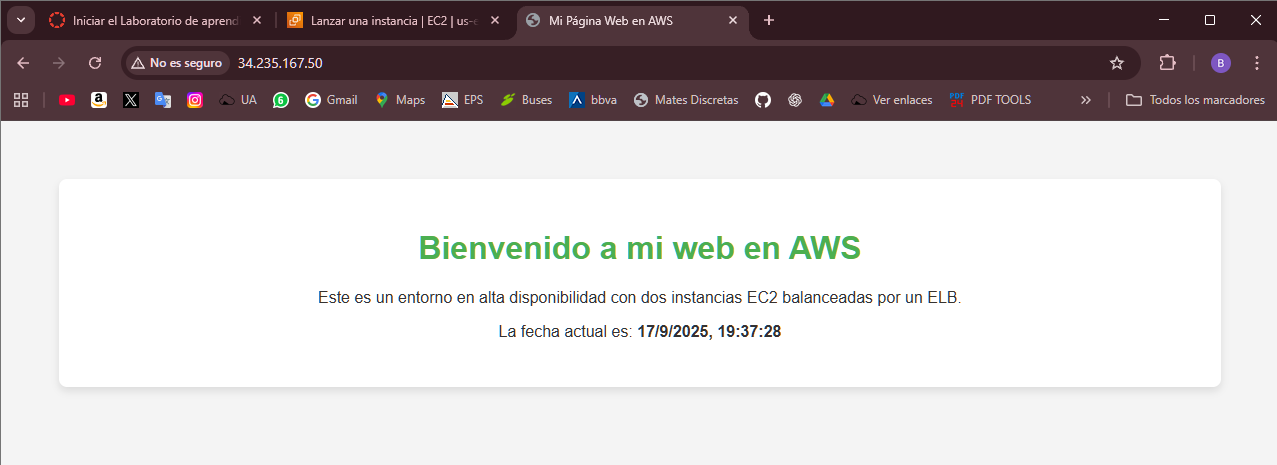
\includegraphics[width=0.95\textwidth]{index.png}
	\caption{http://34.235.167.50/}
	\end{figure}



\newpage


\section{Clonación de la Instancia base mediante AMI}

	Para este apartado debemos de crear una imagen AMI a partir de la instancia base que ya tenemos ejecutando. Esta imagen que usaremos ya tiene instalado httpd, tiene dentro el index.html y el servidor Apache encendido y habilitado. De esta forma no tendremos que conectarnos a ella mediante ssh a no ser que queramos modificar algo.

\subsection{Creación de la AMI}

	Para crear la AMI seleccionamos la instancia de la cual queremos hacer la imagen y le damos a ``Crear imagen'' escribimos un nombre y la guardamos.

	

	\begin{figure}[H]
	\centering
	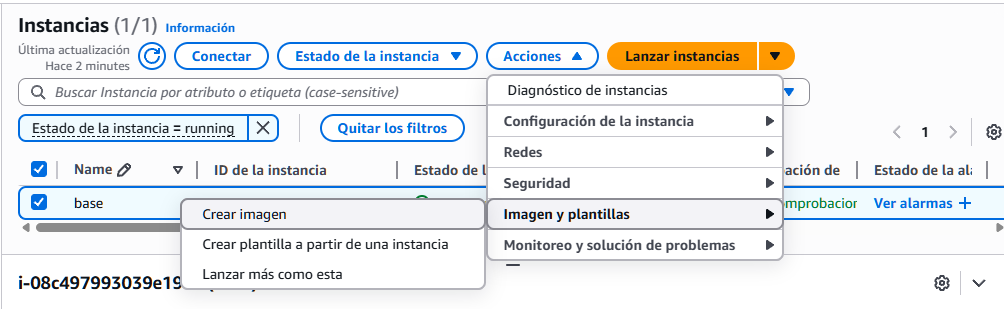
\includegraphics[width=0.95\textwidth]{crear_imagen.png}
	\caption{panel de instancias}
	\end{figure}

\subsection{Instancia a partir de la AMI}
	Una vez que tengamos la AMI debemos de lanzar una instancia nueva a partir de esta para probar su correcto funcionamiento. Esto lo haremos accediendo al menu de ``lanzar instancia'', para esta instancia y en el apartado de 

	
	\begin{figure}[H]
	\centering
	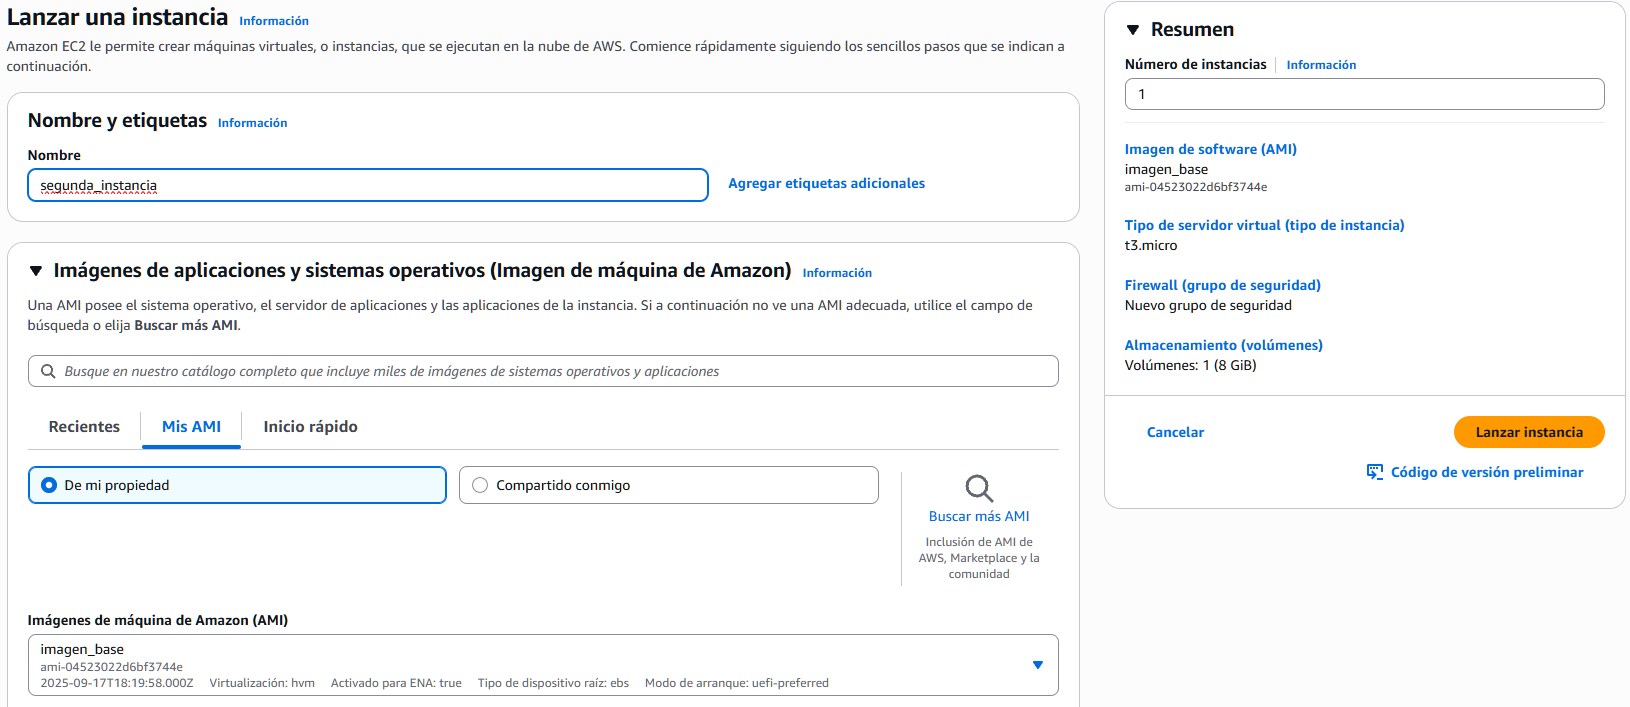
\includegraphics[width=0.95\textwidth]{menu_lanzar_desde_imagen.png}
	\caption{panel de lanzar una instancia}
	\end{figure}

\newpage

\subsection{Acceso Index de la segunda instancia}

	Desde el menu de instancias ya nos aparecerán las dos instancias. Y desde la configuración podremos acceder al ip publico de esta nueva instancia y comprobar si se muestra nuestro index.

	\begin{figure}[H]
	\centering
	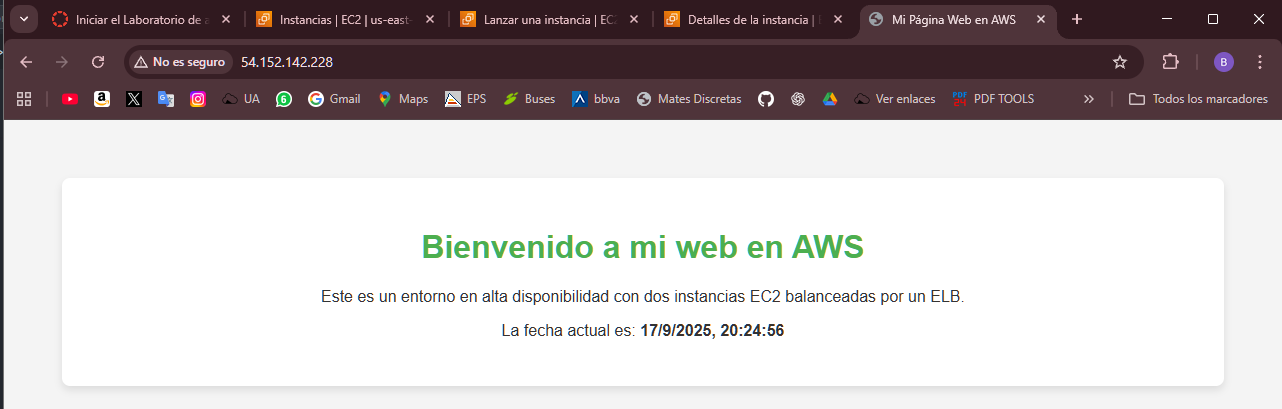
\includegraphics[width=0.95\textwidth]{index2.png}
	\caption{http://54.152.142.228/}
	\end{figure}
\newpage

\section{Configuración de Alta Disponibilidad}
	Para aumentar la disponibilidad de nuestra web es imprescindible usar balanceadores de carga para hacer efectivo el aumento de recursos/instancias. Un balanceador de carga nos permite redirigir el trafico de forma uniforme a las instancias que tengamos ejecutando. 
	

\subsection{Grupo de seguridad}

	Igual que hemos hecho para las instancias, para el balanceador necesitaremos un nuevo grupo de seguridad en el que permitamos entradas http desde cualquier lugar. Como la entrada será a partir de nuestro balanceador, modificaremos también el grupo de seguridad de nuestras instancias para dejar de permitir cualquier entrada http y en su lugar permitiremos la entrada del grupo de seguridad del balanceador. De esta forma lo he hecho yo.

	\begin{figure}[H]
	\centering
	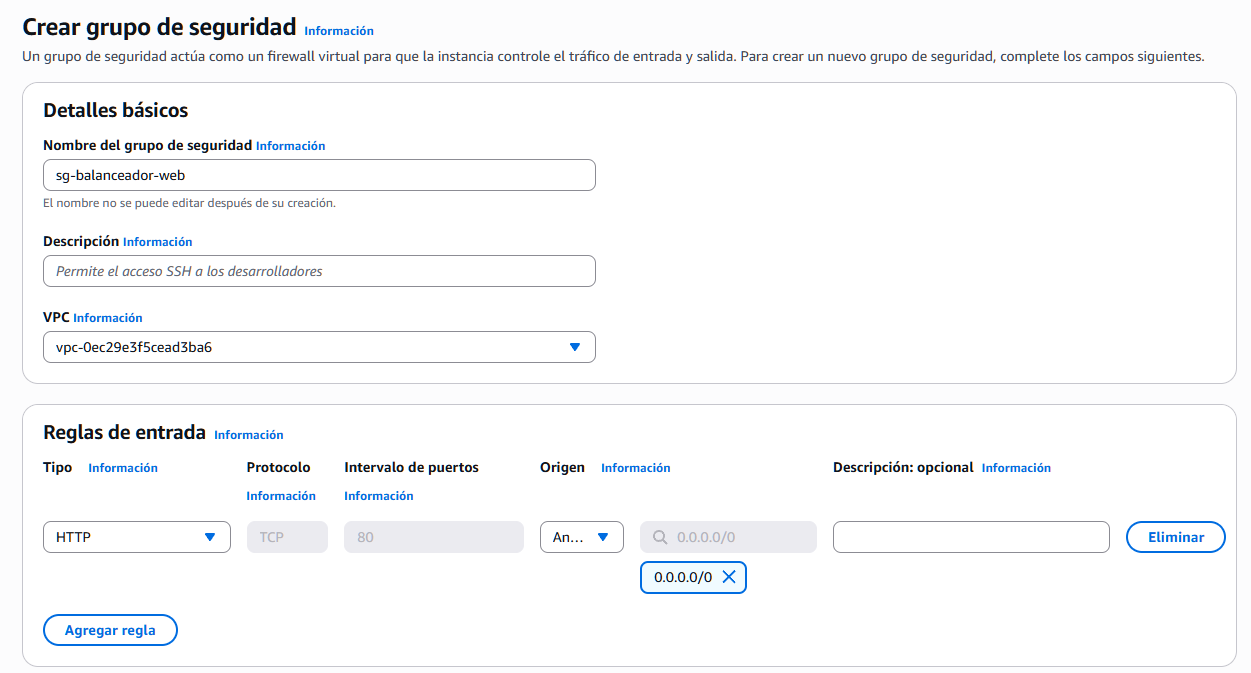
\includegraphics[width=0.95\textwidth]{grupo_de_seguridad_balanceador.png}
	\caption{Grupo de seguridad del balanceador}
	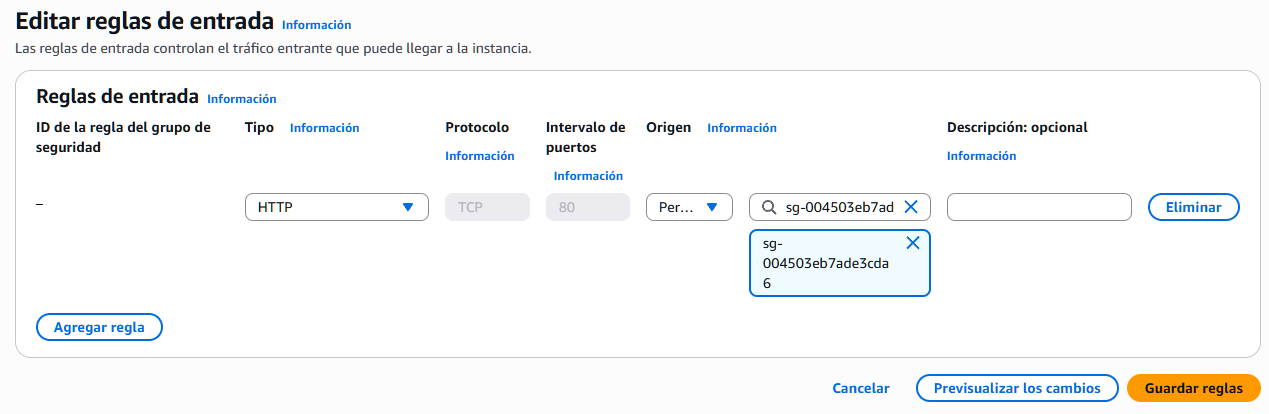
\includegraphics[width=0.95\textwidth]{editar_reglas_grupo_seguridad.png}
	\caption{Grupo de seguridad de las instancias editado}
	\end{figure}

\subsection{Grupo de destino}

	El balanceador de carga necesita aún que agrupemos nuestras instancias para que pueda redirigir el trafico correctamente donde queramos, y esto se hace con un grupo de destino como muestro a continuación.

	\begin{figure}[H]
	\centering
	
\includegraphics[width=0.95\textwidth]{grupo_de_destino.png}
	\caption{Grupo de destino}
	\end{figure}

	Elegimos el tipo de destino instancias y posteriormente insertamos nuestras instancias dentro del grupo, cuando tengamos el grupo de destino y el grupo de seguridad correctamente configurados podremos comenzar a crear nuestro balanceador de carga.


\subsection{Creación del balanceador de carga}

Para crear el balanceador de carga necesitamos entrar a la opción de balanceador de carga de aplicaciones. Al seleccionarla debemos de tener 3 cosas muy claras para configurar bien el balanceador, lo primero sería que debemos de asegurarnos que el esquema sea el de expuesto a internet para poder conectarnos desde cualquier lugar. Lo segundo sería volver al panel de instancias y fijarse en la zona del servidor en el que se estén ejecutando, para que dentro del panel de ``crear balanceador'' elegir la Zona de disponibilidad y subred de estas instancias. Lo último que queda por configurar sería ajustar el grupo de seguridad y el de destino del balanceador, lo hacemos simplemente eligiendo los grupos que hemos creado antes. Cuando le demos a crear ya tendremos ejecutando el balanceador de carga correctamente.

	\begin{figure}[H]
	\centering
	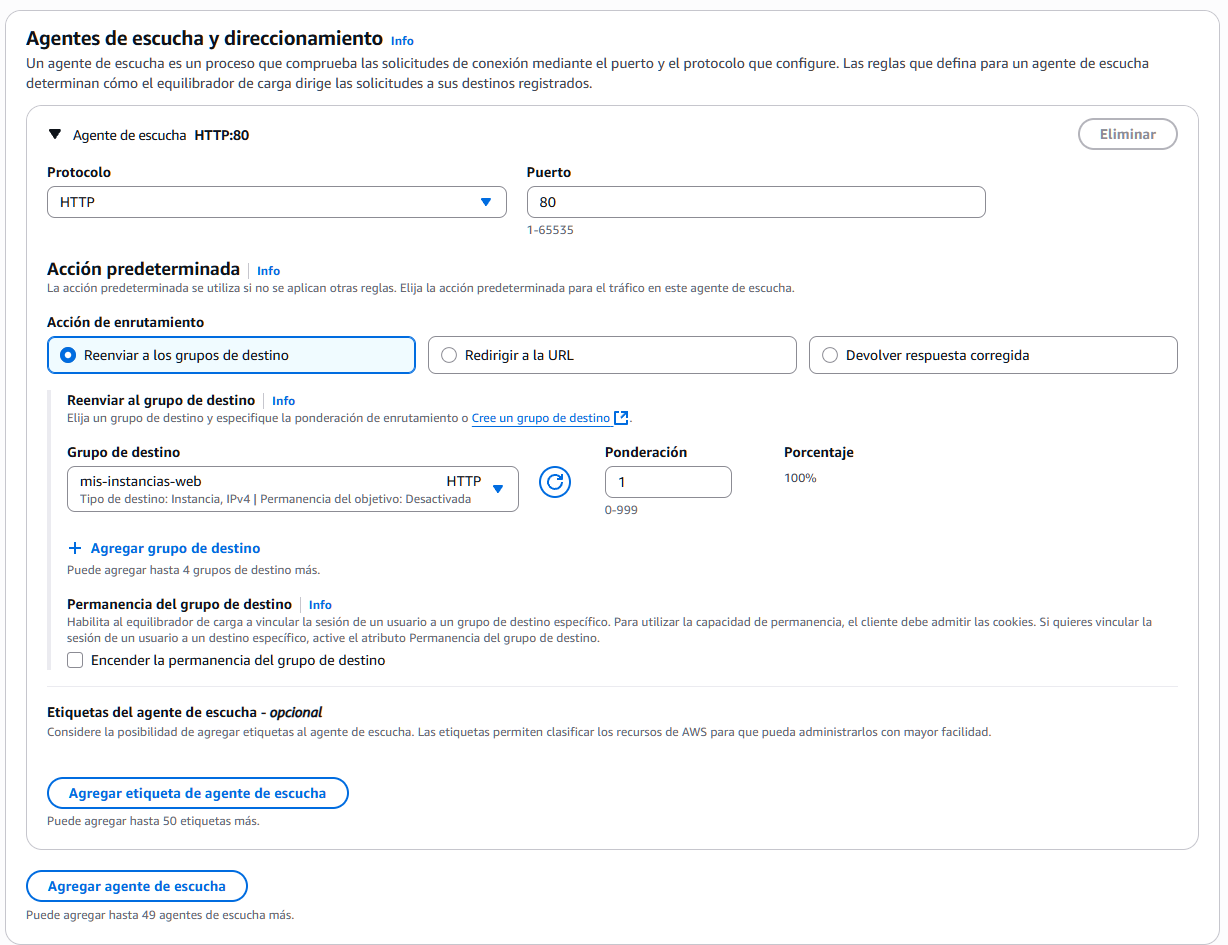
\includegraphics[width=0.95\textwidth]{agentes_de_escucha.png}
	\caption{Configuración de direccionamiento}
	\end{figure}

\section{Pruebas de Alta Disponibilidad}

	Para las pruebas de Alta Disponibilidad debemos de saber a que instancia estamos accediendo, la forma saberlo será desde el mismo index.html de cada página, por lo que, accederemos a nuestras instancias mediante ssh y cambiaremos el mensaje que se muestra para indicar que instancia se esta mostrando. Para comprobarlo modificaremos un momento el grupo de seguridad para poder acceder a cada instancia individualmente.

	\begin{figure}[H]
	\centering
	
\includegraphics[width=0.475\textwidth]{PrimeraInstancia.png}
	
\includegraphics[width=0.475\textwidth]{SegundaInstancia.png}
	\caption{Nuevos dos index.html}
	\end{figure}
	 


\subsection{Prueba de balanceo de carga}
	Al acceder a la URL del balanceador de carga, que se encuentra en el apartado de Nombre de DNS, podemos observar como cada vez que recargamos la página se va alternando el texto de ``esta es la primera o segunda instancia''
	\begin{figure}[H]
	\centering
	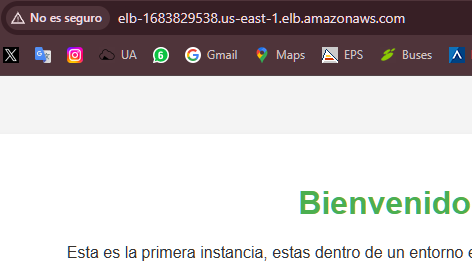
\includegraphics[width=0.475\textwidth]{index_balanceo_1.png}
	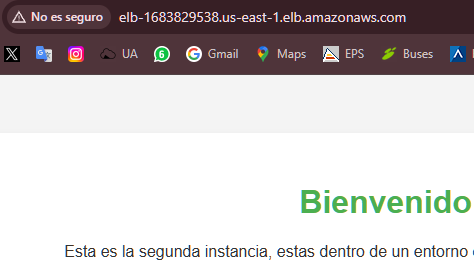
\includegraphics[width=0.475\textwidth]{index_balanceo_2.png}
	\caption{Index balanceador}
	\end{figure}

\subsection{Prueba de fallo de instancia}
	Si detenemos la primera instancia vemos como la pagina web al principio cuando accede a la instancia detenida nos da error 503 pero después de unos segundos recargando todo el trafico se redirige a la segunda instancia y la página sigue funcionando como si no hubiera pasado nada. Si volvemos a a iniciarla vuelve a alternarse al darle al bóton de recargar después de pasar unos segundos.

	\begin{figure}[H]
	\centering
	
\includegraphics[width=0.95\textwidth]{imagen_detenida.png}
	\caption{Imagen detenida}
	\end{figure}

\newpage

\subsection{Prueba de escalabilidad}

	Para probar la escalabilidad del sistema necesitamos crear una nueva instancia a partir de la AMI anterior y modificar el texto del index para poder verificar correctamente que se esta ejecutando la tercera instancia. Primero creamos la instancia con el grupo de seguridad y AMI pertinente. Nos conectamos mediante ssh y cambiamos el mensaje del html. Después agregamos la instancia nueva dándole a registrar destinos y guardando el grupo de destino. Comprobamos el estado del destino dentro de los detalles del grupo y cuando pase de estar inicializando a `Healthy' podemos probar de nuevo si al refrescar la página el servidor se encuentra disponible.


	\begin{figure}[H]
	\centering
	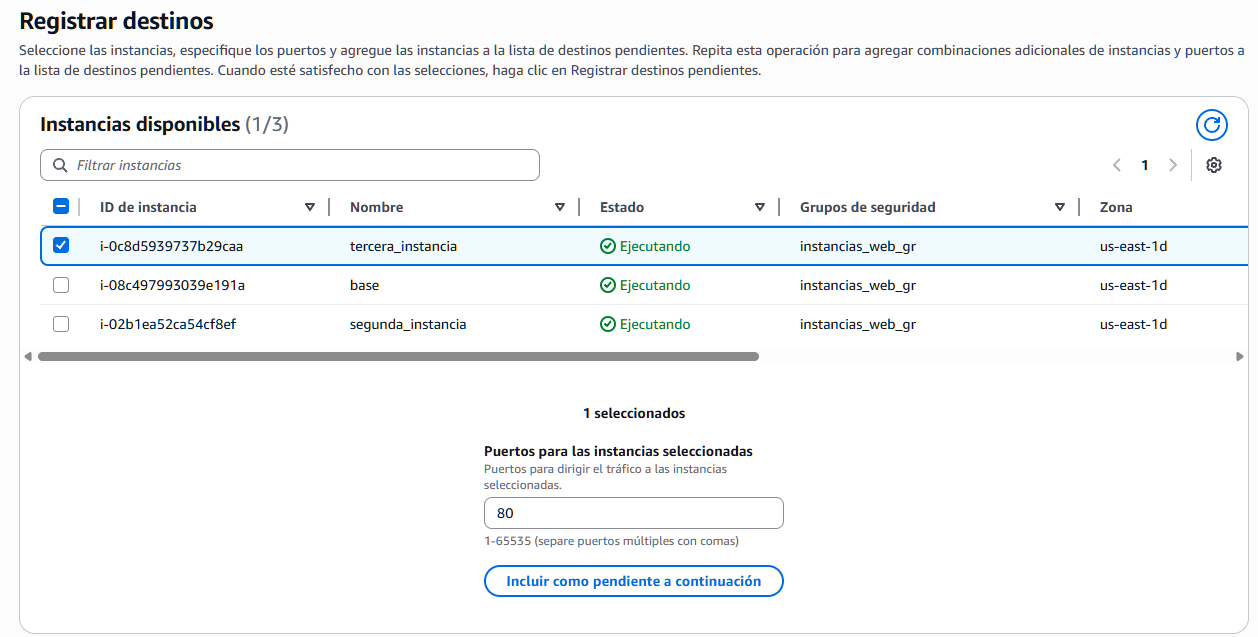
\includegraphics[width=0.95\textwidth]{registrar_destinos.png}
	\caption{Registrar destinos}
	\end{figure}

	\begin{figure}[H]
	\centering
	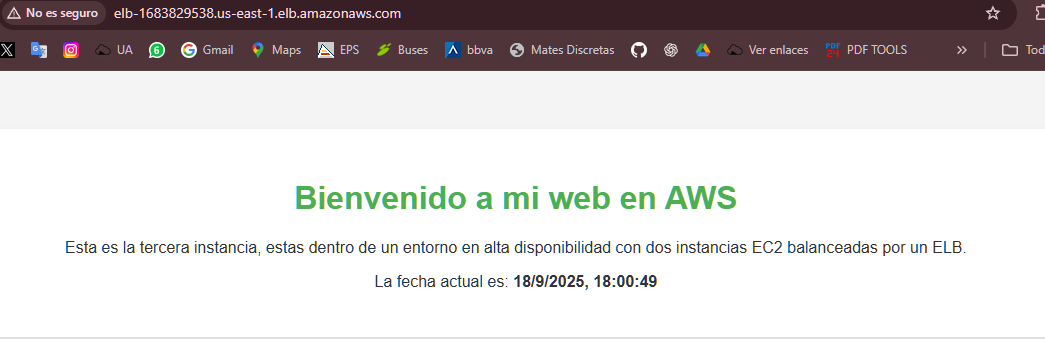
\includegraphics[width=0.95\textwidth]{tercera_instancia_disponible.png}
	\caption{Index tercera instancia}
	\end{figure}

	

\end{document}
